\titreTD{\thenumTD}{Les orbitales hybrides}

\exo{Les diff\'erents types d'hybridation}

Soit les mol\'ecules ci-apr\`es et leur figure de r\'epulsion (FR) selon VSEPR.

\begin{enumerate}[\bf 1)]
\item Quel type d'hybridation pour le \textbf{Si} dans SiH$_4$, pour le \textbf{C} et le \textbf{O} dans le formol 
(H$_2$CO) et pour le \textbf{C} et le \textbf{N} dans l'acide cyanhydrique (HCN) permet d'expliquer les figures de 
r\'epulsion bas\'ees sur la th\'eorie VSEPR~?
\begin{figure}[!h]
\begin{center}
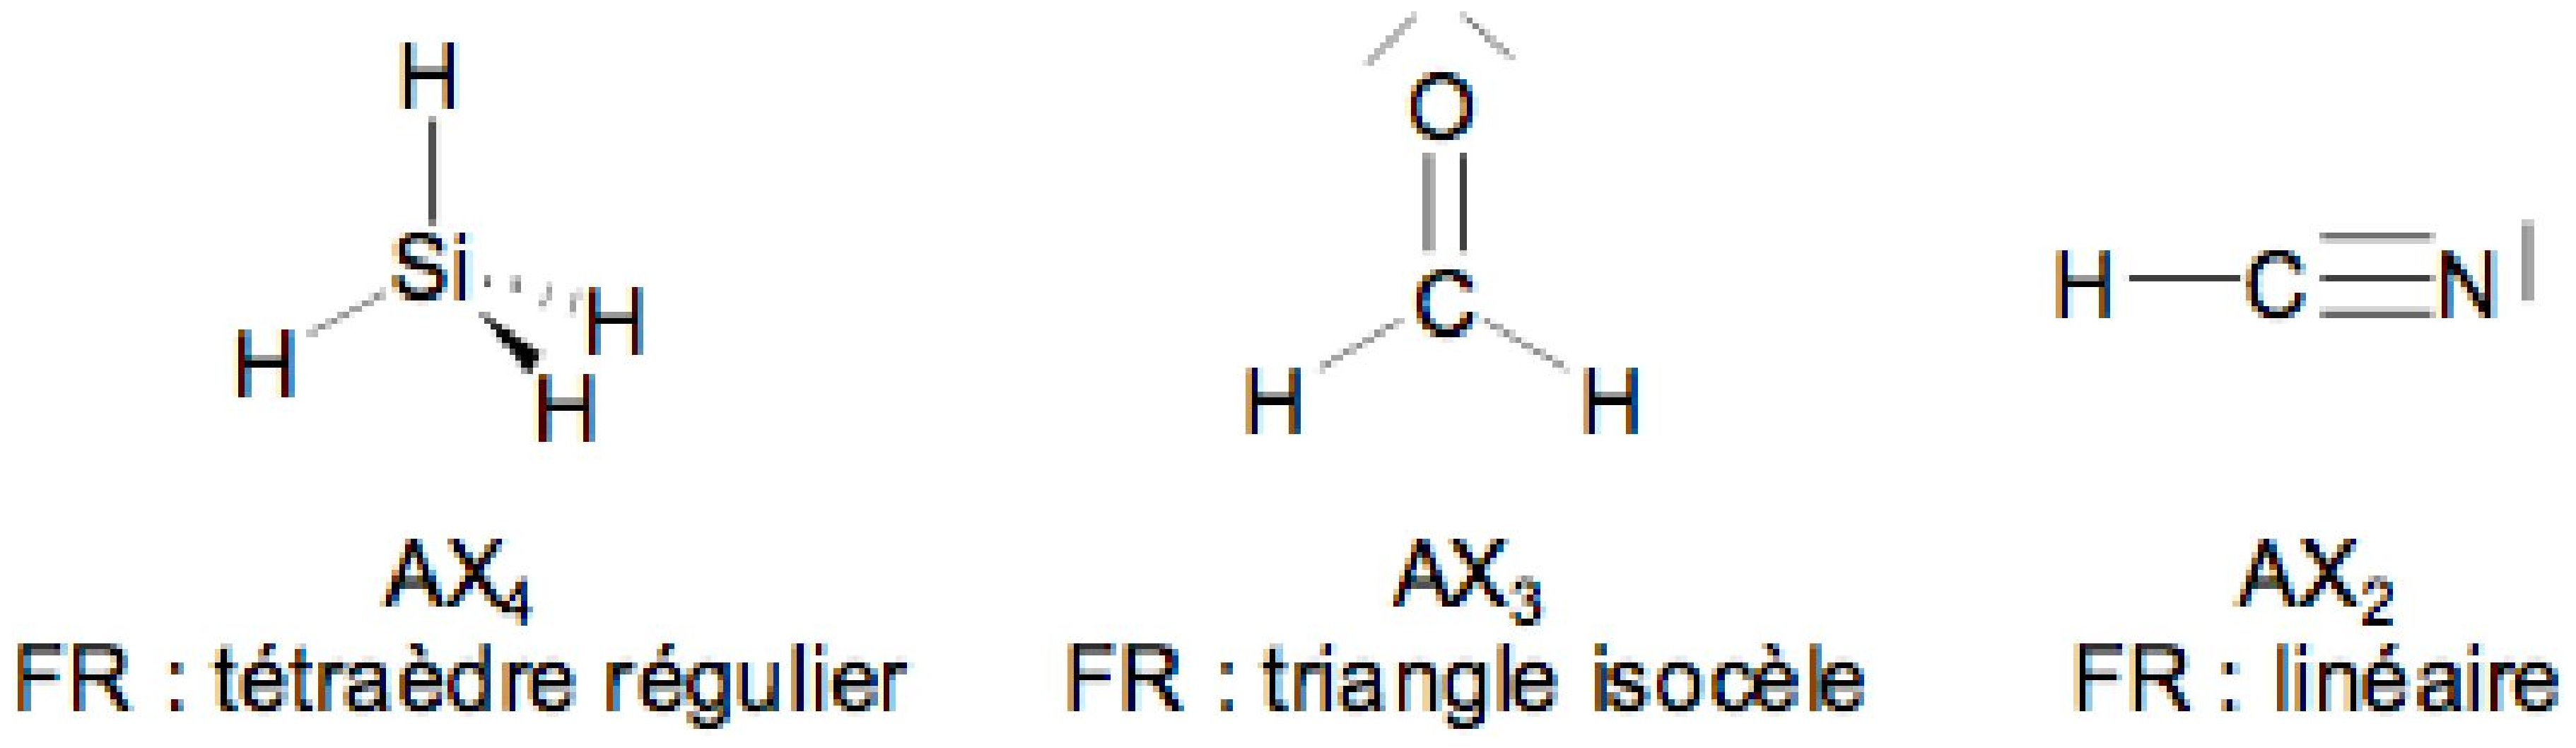
\includegraphics[scale=0.17]{figure/vsepr2.eps}
\end{center}
\end{figure}

\item Dessinez les trois mol\'ecules en faisant appara\^itre les orbitales atomiques hybrides et non hybrides des 
diffi\'erents atomes.
\item Pour chacune des mol\'ecules, donnez les diff\'erents types de liaisons ou 
orbitales mol\'eculaires form\'ees ($\sigma$ ou $\pi$).
\end{enumerate}

\textit{La r\'edaction de l'exercice pourra se faire selon l'exemple donn\'e ci-dessous :}\\
Mol\'ecule d'\'ethyl\`ene~:

%
\begin{figure}[!h]
\begin{center}
\includegraphics[height=2.0cm]{figure/vsepr3.eps}
\end{center}
\end{figure}
%

Ce carbone (1) est entour\'e de trois liaisons selon la th\'eorie VSEPR~: 2 simples, une double. Il est donc de type AX$_3$. 
Couche de valence du carbone : $2s^2 2p^2$.
%
\begin{figure}[!h]
\begin{center}
\includegraphics[height=1.5cm]{figure/vsepr4.eps}
\end{center}
\end{figure}
%

Pour cr\'eer \textbf{3} liaisons autour du carbone il faut \textbf{3} orbitales hybrides~:\\
\textbf{1} orbitale atomique (OA) $s$ + \textbf{2} OA $p$ = \textbf{3} OA hybrides de type $sp^2$.\\
Conclusion, une fois hybrid\'e, le carbone poss\`ede 3 OA hybrides de type $sp^2$ et il lui reste donc une orbitale $p$
non transform\'ee. On peut alors r\'epartir les 4 \'electrons dans ces 4 orbitales de fa\c{c}on \`a former 
les liaisons avec les voisins.
\begin{figure}[!h]
\begin{center}
\includegraphics[height=1.5cm]{figure/vsepr5.eps}
\end{center}
\end{figure}

\clearpage

\textbf{Repr\'esentation}:
OA hybride de type sp$^2$~:     OA de type $p$ restante (remarque: on obtient le mi\^eme r\'esultat pour le carbone 2)
\begin{figure}[!h]
\begin{center}
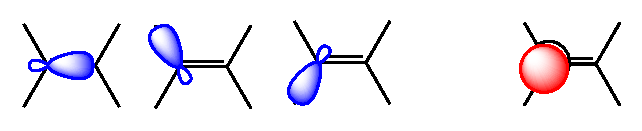
\includegraphics[height=1.5cm]{figure/vsepr6.eps}
\end{center}
\end{figure}

\textbf{Repr\'esentation} du carbone 1~: 
%3 OA hybrides de type $sp^2$ et une OA de type $p$ 
%(remarque: on obtient le mi\^eme r\'esultat pour le carbone 2) - 
Approche des hydrog\`enes -- Visualisation des diff\'erentes 
liaisons ou orbitales moli\'eculaires (OM) form\'ees.
\begin{figure}[!h]
\begin{center}
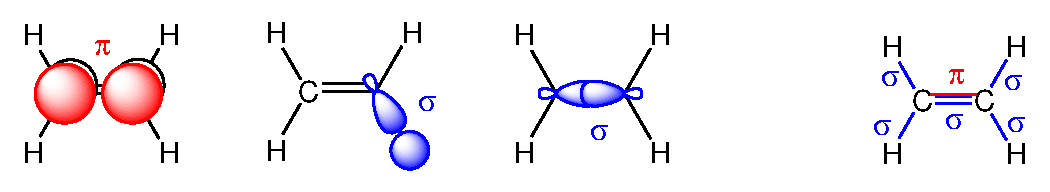
\includegraphics[height=2.5cm]{figure/vsepr7.eps}
\end{center}
\end{figure}


\exo{Hybridation}
\begin{enumerate}[\bf 1)]
\item Exemple de H-Be-H (mol\'ecule lin\'eaire, $sp$)\\
Une orbitale hybride $sp$ se construit en combinant une orbitale $s$ et une orbitale $p$ d'un m\^eme atome (ici Be). 
Pour un tel couple, on peut former 2 hybrides $sp$.
\begin{enumerate}
\item Repr\'esentez sch\'ematiquement chacune de ces 2 hybrides (un dessin par orbitale).
\item Combien d'orbitales $p$ restent pures sur Be~?
Les dessiner (un dessin par orbitale).
\end{enumerate}
\item Exemple de CH$_3^+$ (cation triangulaire, $sp^2$)\\
Les orbitales hybrides $sp^2$ sont construites par la combinaison d'une orbitale $s$ et de 2 orbitales $p$ d'un m\^eme atome (ici C).
\begin{enumerate}
\item Dessinez chacune de ces 3 hybrides (un dessin par orbitale).
\item Combien d'orbitales $p$ restent pures sur C~?
Les dessiner (un dessin par orbitale).
\end{enumerate}
\end{enumerate}
